% ============================================================================
% CHƯƠNG 3: VECTOR SUM VÀ MATRIX SUM
% ============================================================================
\chapter{Vector Sum và Matrix Sum}
\label{chap:vector_matrix}

\section{Bài toán Vector Sum (Cộng hai Vector)}

\subsection{Mô tả bài toán}

Cho hai vector $A$ và $B$ có cùng kích thước $n$, tính vector $C$ sao cho:
\begin{equation}
C[i] = A[i] + B[i], \quad \forall i \in [0, n-1]
\end{equation}

Đây là bài toán \textbf{embarrassingly parallel} - mỗi phép cộng hoàn toàn độc lập, không cần đồng bộ giữa các threads.

\begin{figure}[H]
\centering
\begin{tikzpicture}[scale=0.8]
    % Vector A
    \node[left] at (-0.5, 2) {\textbf{A:}};
    \foreach \i/\v in {0/3.1, 1/2.4, 2/5.7, 3/1.2, 4/4.8, 5/...} {
        \draw[fill=blue!20] (\i*1.2, 1.7) rectangle ++(1,0.6);
        \node[font=\footnotesize] at ({\i*1.2+0.5}, 2) {\v};
    }
    
    % Plus sign
    \node[font=\Huge] at (3.5, 1) {+};
    
    % Vector B
    \node[left] at (-0.5, 0.3) {\textbf{B:}};
    \foreach \i/\v in {0/1.5, 1/3.2, 2/2.1, 3/4.5, 4/0.9, 5/...} {
        \draw[fill=green!20] (\i*1.2, 0) rectangle ++(1,0.6);
        \node[font=\footnotesize] at ({\i*1.2+0.5}, 0.3) {\v};
    }
    
    % Equals sign
    \node[font=\Huge] at (3.5, -0.8) {=};
    
    % Vector C
    \node[left] at (-0.5, -1.4) {\textbf{C:}};
    \foreach \i/\v in {0/4.6, 1/5.6, 2/7.8, 3/5.7, 4/5.7, 5/...} {
        \draw[fill=red!20] (\i*1.2, -1.7) rectangle ++(1,0.6);
        \node[font=\footnotesize] at ({\i*1.2+0.5}, -1.4) {\v};
    }
    
    % Thread assignment
    \foreach \i in {0,...,4} {
        \draw[dashed, gray] ({\i*1.2+0.5}, 1.7) -- ({\i*1.2+0.5}, -1.7);
        \node[font=\tiny, gray] at ({\i*1.2+0.5}, -2.2) {T\i};
    }
    
    \node[font=\footnotesize] at (3.5, -2.8) {Mỗi thread xử lý một phần tử};
\end{tikzpicture}
\caption{Minh họa bài toán Vector Sum}
\label{fig:vector_sum}
\end{figure}

\subsection{Cài đặt trên Host (CPU)}

\begin{lstlisting}[caption={Vector Sum tuần tự trên CPU}, label={lst:vector_sum_cpu}]
void sumHost(float *a, float *b, float *c, int n) {
    for (int i = 0; i < n; i++) {
        c[i] = a[i] + b[i];
    }
}
\end{lstlisting}

\subsection{Cài đặt Kernel CUDA}

\begin{lstlisting}[caption={Vector Sum Kernel trên GPU}, label={lst:vector_sum_gpu}]
__global__ void sumDevice(float *a, float *b, float *c, int n) {
    // Tinh chi so global cua thread
    int i = blockIdx.x * blockDim.x + threadIdx.x;
    
    // Kiem tra bien - QUAN TRONG de tranh loi truy cap bo nho
    if (i < n) {
        c[i] = a[i] + b[i];
    }
}
\end{lstlisting}

\subsection{Chương trình hoàn chỉnh}

\begin{lstlisting}[caption={Chương trình Vector Sum đầy đủ}, label={lst:vector_sum_full}]
#include <cuda_runtime.h>
#include <stdio.h>
#include <stdlib.h>
#include <time.h>
#include <sys/time.h>

#define BLOCK_SIZE 256

// Ham do thoi gian
double cpuSecond() {
    struct timeval tp;
    gettimeofday(&tp, NULL);
    return ((double)tp.tv_sec + (double)tp.tv_usec * 1.e-6);
}

// Khoi tao du lieu ngau nhien
void initData(float *ip, int size) {
    srand(time(NULL));
    for (int i = 0; i < size; i++) {
        ip[i] = (float)(rand() & 0xFF) / 10.0f;
    }
}

// Kernel: Vector Sum tren Device
__global__ void sumDevice(float *a, float *b, float *c, int n) {
    int i = blockIdx.x * blockDim.x + threadIdx.x;
    if (i < n) {
        c[i] = a[i] + b[i];
    }
}

// Ham kiem tra ket qua
void checkResult(float *hostRef, float *gpuRef, const int N) {
    double epsilon = 1.0E-8;
    for (int i = 0; i < N; i++) {
        if (abs(hostRef[i] - gpuRef[i]) > epsilon) {
            printf("Mismatch at %d: Host %f vs GPU %f\n", 
                   i, hostRef[i], gpuRef[i]);
            return;
        }
    }
    printf("Ket qua CHINH XAC!\n");
}

void sumHost(float *a, float *b, float *c, int n) {
    for (int i = 0; i < n; i++) c[i] = a[i] + b[i];
}

int main() {
    printf("=== Vector Sum ===\n");

    // 1. Thiet lap kich thuoc
    int n = 1 << 24;  // ~16 trieu phan tu
    size_t nBytes = n * sizeof(float);
    printf("Vector size: %d elements (%.2f MB)\n", n, nBytes/1e6);

    // 2. Cap phat bo nho Host
    float *hA = (float *)malloc(nBytes);
    float *hB = (float *)malloc(nBytes);
    float *hostRef = (float *)malloc(nBytes);
    float *gpuRef = (float *)malloc(nBytes);

    // 3. Khoi tao du lieu
    initData(hA, n);
    initData(hB, n);

    // 4. Cap phat bo nho Device
    float *dA, *dB, *dC;
    cudaMalloc((void **)&dA, nBytes);
    cudaMalloc((void **)&dB, nBytes);
    cudaMalloc((void **)&dC, nBytes);

    // 5. Copy du lieu Host -> Device
    cudaMemcpy(dA, hA, nBytes, cudaMemcpyHostToDevice);
    cudaMemcpy(dB, hB, nBytes, cudaMemcpyHostToDevice);

    // 6. Cau hinh Kernel
    dim3 block(BLOCK_SIZE);
    dim3 grid((n + block.x - 1) / block.x);
    printf("Config: <<<%d, %d>>>\n", grid.x, block.x);

    // 7. Chay Kernel va do thoi gian
    double iStart = cpuSecond();
    sumDevice<<<grid, block>>>(dA, dB, dC, n);
    cudaDeviceSynchronize();
    double iElaps = cpuSecond() - iStart;
    printf("GPU Time: %.4f ms\n", iElaps * 1000);

    // 8. Copy ket qua Device -> Host
    cudaMemcpy(gpuRef, dC, nBytes, cudaMemcpyDeviceToHost);

    // 9. Kiem tra ket qua
    sumHost(hA, hB, hostRef, n);
    checkResult(hostRef, gpuRef, n);

    // 10. Giai phong bo nho
    cudaFree(dA); cudaFree(dB); cudaFree(dC);
    free(hA); free(hB); free(hostRef); free(gpuRef);

    return 0;
}
\end{lstlisting}

\subsection{Phân tích hiệu năng}

\begin{table}[H]
\centering
\caption{So sánh hiệu năng Vector Sum với các Block Size khác nhau}
\label{tab:vector_sum_perf}
\begin{tabular}{@{}ccccc@{}}
\toprule
\textbf{Vector Size} & \textbf{Block Size} & \textbf{Grid Size} & \textbf{GPU Time (ms)} & \textbf{Bandwidth (GB/s)} \\
\midrule
$2^{24}$ & 32 & 524288 & 12.45 & 32.2 \\
$2^{24}$ & 128 & 131072 & 5.67 & 70.7 \\
$2^{24}$ & 256 & 65536 & 4.23 & 94.8 \\
$2^{24}$ & 512 & 32768 & 4.89 & 82.0 \\
$2^{24}$ & 1024 & 16384 & 6.12 & 65.5 \\
\bottomrule
\end{tabular}
\end{table}

\textbf{Nhận xét:}
\begin{itemize}
    \item Block size 256 cho hiệu năng tốt nhất trong ví dụ này
    \item Quá nhỏ (32): Không tận dụng hết tài nguyên SM
    \item Quá lớn (1024): Giảm số active blocks, giảm occupancy
\end{itemize}

\section{Bài toán Matrix Sum (Cộng hai Ma trận)}

\subsection{Mô tả bài toán}

Cho hai ma trận $A$ và $B$ có kích thước $M \times N$, tính ma trận $C$:
\begin{equation}
C[i][j] = A[i][j] + B[i][j], \quad \forall i \in [0, M-1], j \in [0, N-1]
\end{equation}

\subsection{Ánh xạ 2D}

Sử dụng Grid và Block 2D để ánh xạ tự nhiên vào ma trận:

\begin{figure}[H]
\centering
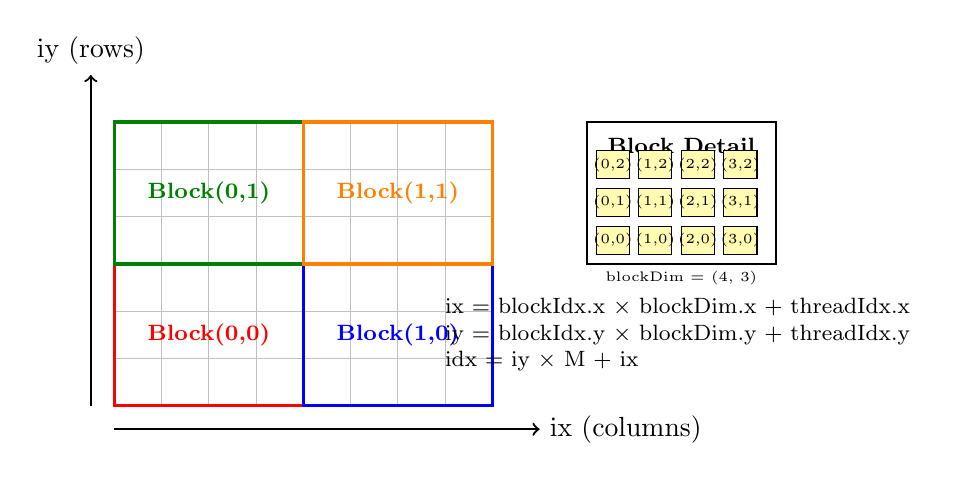
\begin{tikzpicture}[scale=0.6]
    % Matrix representation
    \draw[step=1, gray!50, thin] (0,0) grid (8,6);
    
    % Block boundaries
    \draw[very thick, red] (0,0) rectangle (4,3);
    \draw[very thick, blue] (4,0) rectangle (8,3);
    \draw[very thick, green!50!black] (0,3) rectangle (4,6);
    \draw[very thick, orange] (4,3) rectangle (8,6);
    
    % Block labels
    \node[red, font=\footnotesize\bfseries] at (2,1.5) {Block(0,0)};
    \node[blue, font=\footnotesize\bfseries] at (6,1.5) {Block(1,0)};
    \node[green!50!black, font=\footnotesize\bfseries] at (2,4.5) {Block(0,1)};
    \node[orange, font=\footnotesize\bfseries] at (6,4.5) {Block(1,1)};
    
    % Axes
    \draw[thick, ->] (0,-0.5) -- (9,-0.5) node[right] {ix (columns)};
    \draw[thick, ->] (-0.5,0) -- (-0.5,7) node[above] {iy (rows)};
    
    % Thread detail
    \draw[thick] (10,3) rectangle (14,6);
    \node[font=\footnotesize\bfseries] at (12,5.5) {Block Detail};
    \foreach \x in {0,1,2,3} {
        \foreach \y in {0,1,2} {
            \draw[fill=yellow!30] ({10.2+\x*0.9}, {3.2+\y*0.8}) rectangle ++(0.7,0.6);
            \node[font=\tiny] at ({10.55+\x*0.9}, {3.5+\y*0.8}) {(\x,\y)};
        }
    }
    \node[font=\tiny] at (12, 2.7) {blockDim = (4, 3)};
    
    % Index formula
    \node[font=\footnotesize, text width=6cm] at (12, 1.5) {
        ix = blockIdx.x $\times$ blockDim.x + threadIdx.x\\
        iy = blockIdx.y $\times$ blockDim.y + threadIdx.y\\
        idx = iy $\times$ M + ix
    };
\end{tikzpicture}
\caption{Ánh xạ 2D Block/Thread vào ma trận}
\label{fig:matrix_mapping}
\end{figure}

\subsection{Cài đặt Kernel 2D}

\begin{lstlisting}[caption={Matrix Sum Kernel với Block 2D}, label={lst:matrix_sum_kernel}]
// m: so cot (width), n: so hang (height)
__global__ void matrixSum(float *a, float *b, float *c, int m, int n) {
    // Tinh chi so 2D
    int ix = threadIdx.x + blockIdx.x * blockDim.x;
    int iy = threadIdx.y + blockIdx.y * blockDim.y;
    
    // Chuyen sang chi so 1D (row-major layout)
    int idx = iy * m + ix;

    // Kiem tra bien 2 chieu
    if (ix < m && iy < n) {
        c[idx] = a[idx] + b[idx];
    }
}
\end{lstlisting}

\subsection{Chương trình hoàn chỉnh}

\begin{lstlisting}[caption={Matrix Sum - Chương trình đầy đủ}, label={lst:matrix_sum_full}]
#include <cuda_runtime.h>
#include <stdio.h>
#include <sys/time.h>

#define DIM_X 32
#define DIM_Y 32

double cpuSecond() {
    struct timeval tp;
    gettimeofday(&tp, NULL);
    return ((double)tp.tv_sec + (double)tp.tv_usec * 1.e-6);
}

void initData(float *ip, int size) {
    srand(time(NULL));
    for (int i = 0; i < size; i++) {
        ip[i] = (float)(rand() & 0xFF) / 10.0f;
    }
}

__global__ void sumDevice(float *a, float *b, float *c, int m, int n) {
    int ix = threadIdx.x + blockIdx.x * blockDim.x;
    int iy = threadIdx.y + blockIdx.y * blockDim.y;
    int idx = iy * m + ix;

    if (ix < m && iy < n) {
        c[idx] = a[idx] + b[idx];
    }
}

void checkResult(float *hostRef, float *gpuRef, int size) {
    double epsilon = 1.0E-8;
    for (int i = 0; i < size; i++) {
        if (abs(hostRef[i] - gpuRef[i]) > epsilon) {
            printf("Mismatch at %d\n", i);
            return;
        }
    }
    printf("Ket qua CHINH XAC!\n");
}

void sumHost(float *a, float *b, float *c, int size) {
    for (int i = 0; i < size; i++) c[i] = a[i] + b[i];
}

int main() {
    printf("=== Matrix Sum ===\n");

    // Kich thuoc ma tran
    int m = 1 << 12;  // 4096 columns
    int n = 1 << 12;  // 4096 rows
    int size = m * n;
    size_t nBytes = size * sizeof(float);
    printf("Matrix: %d x %d (%.2f MB)\n", n, m, nBytes/1e6);

    // Host memory
    float *hA = (float *)malloc(nBytes);
    float *hB = (float *)malloc(nBytes);
    float *hostRef = (float *)malloc(nBytes);
    float *gpuRef = (float *)malloc(nBytes);

    initData(hA, size);
    initData(hB, size);

    // Device memory
    float *dA, *dB, *dC;
    cudaMalloc((void **)&dA, nBytes);
    cudaMalloc((void **)&dB, nBytes);
    cudaMalloc((void **)&dC, nBytes);

    cudaMemcpy(dA, hA, nBytes, cudaMemcpyHostToDevice);
    cudaMemcpy(dB, hB, nBytes, cudaMemcpyHostToDevice);

    // Cau hinh 2D
    dim3 block(DIM_X, DIM_Y);
    dim3 grid((m + block.x - 1) / block.x, 
              (n + block.y - 1) / block.y);

    printf("Block: (%d, %d), Grid: (%d, %d)\n", 
           block.x, block.y, grid.x, grid.y);

    // Chay kernel
    double iStart = cpuSecond();
    sumDevice<<<grid, block>>>(dA, dB, dC, m, n);
    cudaDeviceSynchronize();
    double iElaps = cpuSecond() - iStart;
    printf("GPU Time: %.4f ms\n", iElaps * 1000);

    // Kiem tra
    cudaMemcpy(gpuRef, dC, nBytes, cudaMemcpyDeviceToHost);
    sumHost(hA, hB, hostRef, size);
    checkResult(hostRef, gpuRef, size);

    // Giai phong
    cudaFree(dA); cudaFree(dB); cudaFree(dC);
    free(hA); free(hB); free(hostRef); free(gpuRef);

    return 0;
}
\end{lstlisting}

\subsection{So sánh các cấu hình Block 2D}

\begin{table}[H]
\centering
\caption{Hiệu năng Matrix Sum với các cấu hình Block khác nhau}
\label{tab:matrix_sum_configs}
\begin{tabular}{@{}cccc@{}}
\toprule
\textbf{Block Config} & \textbf{Threads/Block} & \textbf{Time (ms)} & \textbf{Ghi chú} \\
\midrule
(8, 8) & 64 & 8.45 & Occupancy thấp \\
(16, 16) & 256 & 4.12 & Cân bằng tốt \\
(32, 8) & 256 & 4.08 & Tối ưu memory coalescing \\
(32, 16) & 512 & 3.95 & Hiệu năng cao \\
(32, 32) & 1024 & 4.21 & Giới hạn registers \\
\bottomrule
\end{tabular}
\end{table}

\begin{figure}[H]
\centering
\begin{tikzpicture}
\begin{axis}[
    width=12cm,
    height=7cm,
    xlabel={Cấu hình Block},
    ylabel={Thời gian (ms)},
    ymin=0,
    symbolic x coords={(8x8), (16x16), (32x8), (32x16), (32x32)},
    xtick=data,
    nodes near coords,
    nodes near coords align={vertical},
    ybar,
    bar width=20pt,
    fill=cudablue!60,
    title={So sánh hiệu năng Matrix Sum}
]
\addplot coordinates {
    ((8x8), 8.45)
    ((16x16), 4.12)
    ((32x8), 4.08)
    ((32x16), 3.95)
    ((32x32), 4.21)
};
\end{axis}
\end{tikzpicture}
\caption{Biểu đồ so sánh thời gian thực thi Matrix Sum}
\label{fig:matrix_sum_chart}
\end{figure}

\section{Boundary Check - Kiểm tra biên}

\subsection{Tại sao cần Boundary Check?}

Khi số phần tử không chia hết cho block size, sẽ có threads "thừa":

\begin{figure}[H]
\centering
\begin{tikzpicture}[scale=0.7]
    % Array elements
    \foreach \i in {0,...,9} {
        \draw[fill=green!30] (\i*1.1, 0) rectangle ++(1, 0.8);
        \node[font=\footnotesize] at ({\i*1.1+0.5}, 0.4) {\i};
    }
    
    % Invalid elements
    \foreach \i in {10,11} {
        \draw[fill=red!30, pattern=north east lines] (\i*1.1, 0) rectangle ++(1, 0.8);
        \node[font=\footnotesize, red] at ({\i*1.1+0.5}, 0.4) {X};
    }
    
    % Block boundaries
    \draw[very thick, blue] (0, -0.2) rectangle (4.4, 1);
    \draw[very thick, blue] (4.4, -0.2) rectangle (8.8, 1);
    \draw[very thick, blue, dashed] (8.8, -0.2) rectangle (13.2, 1);
    
    \node[font=\footnotesize] at (2.2, -0.6) {Block 0};
    \node[font=\footnotesize] at (6.6, -0.6) {Block 1};
    \node[font=\footnotesize, red] at (11, -0.6) {Block 2 (partial)};
    
    % Legend
    \node[font=\footnotesize] at (6.5, -1.5) {n = 10, blockSize = 4, gridSize = 3};
    \node[font=\footnotesize] at (6.5, -2.2) {Threads 10, 11 sẽ truy cập bộ nhớ không hợp lệ nếu không kiểm tra!};
\end{tikzpicture}
\caption{Vấn đề Boundary khi n không chia hết cho blockSize}
\label{fig:boundary_issue}
\end{figure}

\subsection{Cài đặt Boundary Check}

\begin{lstlisting}[caption={Boundary Check trong kernel}, label={lst:boundary_check}]
__global__ void safeKernel(float *data, int n) {
    int idx = blockIdx.x * blockDim.x + threadIdx.x;
    
    // QUAN TRONG: Kiem tra bien truoc khi truy cap
    if (idx < n) {
        data[idx] = data[idx] * 2.0f;
    }
    // Threads co idx >= n se khong lam gi (thoat som)
}

// Tinh grid size dam bao du cho tat ca phan tu
dim3 block(256);
dim3 grid((n + block.x - 1) / block.x);  // Lam tron len
// Hoac: (n + 255) / 256
\end{lstlisting}

\section{Kết luận chương}

Chương này đã trình bày hai bài toán cơ bản:

\textbf{Vector Sum:}
\begin{itemize}
    \item Sử dụng Grid/Block 1D
    \item Mỗi thread xử lý một phần tử
    \item Block size 256 thường cho hiệu năng tốt
\end{itemize}

\textbf{Matrix Sum:}
\begin{itemize}
    \item Sử dụng Grid/Block 2D để ánh xạ tự nhiên
    \item Công thức index: \code{idx = iy * width + ix}
    \item Cấu hình (32, 16) hoặc (32, 8) tối ưu memory coalescing
\end{itemize}

\textbf{Bài học quan trọng:}
\begin{itemize}
    \item Luôn kiểm tra biên (boundary check) trước khi truy cập bộ nhớ
    \item Thử nghiệm với nhiều cấu hình để tìm tối ưu
    \item Đo thời gian chính xác với CUDA Events hoặc \code{cudaDeviceSynchronize()}
\end{itemize}
